Case study: Boston Housing: Old

\begin{comment}
We perform two case studies to show the efficacy of the visual analysis and refinement tool described in section \ref{sec:implementation:vis}
These case studies use the python implementation described throughout section \ref{sec:implementation}.
We use two datasets, one for each study: Boston housing \cite{belsley2005regression} and Adult income \cite{kohavi1996scaling}.
The goal in the case studies is to analyze a given machine learning model's behavior with respect to a fairness specification, and then decide whether or not to refine the specification or model.
Through these studies we highlight the need for context during refinement, and demonstrate how our analysis tool provides that context.
\end{comment}

\begin{comment}
\subsection{Case Study A: Boston Housing}
\pmcomment{Output of LR model is real-valued, continuous. Needs to be converted to a binary value}
\label{sec:casestudy:boston}
\begin{figure*}[t]
  \centering
  \includegraphics[width=\linewidth]{boston-vis.pdf}
  \caption{A snapshot of our visual analysis tool being used for the case study in section \ref{sec:casestudy:boston}. Here we see observations of areas without low status (the plot on the bottom right) were not made during a decline in the proportion of expectations (the top right plot). Thus violations during this time may be due to a set of observations that is not representative.}
  \label{fig:casestudy:boston}
  \Description{Describe}
\end{figure*}


The dataset we use in this case study is the Boston housing dataset \cite{belsley2005regression}, which details towns in Boston and their corresponding median house cost.
We consider a linear regression model for this case study. The model is trained to predict the median value of owner occupied homes given data for a town in Boston.
We leave 20 data points out as a test set of simulated observations and train on the rest. 
The specification we start our analysis with is a group fairness property that specifies that the expected housing cost in areas with a low status population should be no less than 0.6 times the expected cost of housing in areas that do not have a low status population.
The specification is given below, where r is the return value of our model, which in this case is median house cost:

\begin{lstlisting}[columns=flexible, language=Python]
    @spec(E[r | low_status] / E[r | !low_status] > 0.6)
\end{lstlisting}
We define an area as having a low status population if the percentage of lower status population in the area is less than 12\%. This is reflected in figure \ref{fig:casestudy:boston} where predicates such as \texttt{lstat < 12} are used.

Given the specification, we would now like to use application described in section \ref{sec:implementation:vis} to help determine if our model is likely to adhere to our defined fairness property, and possibly adjust the property according to our findings.
We start the analysis by selecting our desired dataset, model, and finally the specification.
Using the test set, A series of observations are provided to the model.
Although this test set is not necessarily representative of the distribution that will be seen in the wild, it provides a useful simulation for estimating how our model will behave with respect to the specification.

When the simulation has finished we are provided with the tree-like visualization of our specification.
We start by looking at the evaluation plot for the full specification at the root node.
The top level specification is an inequality which evaluates to true (1) when the specification is being adhered to, and false (0) when the specification is being violated.
In this case study, we found that between observations 4 and 8, the specification was being violated.
This should mean that the expected housing cost of low status areas is less than 0.6 times that of areas that are not low status.
We confirm this by looking at the node in the next level of the tree that corresponds to the proportion of expected median housing costs.
The evaluation plot for the proportion (shown in figure \ref{fig:casestudy:boston}) shows the rapid decline that leads to the violation.
This violation could be indicative of unwanted bias in our model, so we analyze further to better understand this behavior.
With the evaluation plot of the proportion shown at the top, we select the node relating to the expected median housing cost in areas that are not low status.
This state of the visualization is shown in figure \ref{fig:casestudy:boston}.
The evaluation plot of the expected cost in areas with low status shows that during the time of the violation, data without low status was not being observed.
As more data is observed (with and without low status), the proportion appears to rise and converge above the threshold.

With these insights we can assume that the violation of our specification was a result of the data being observed during the violation not being representative of the population.
If this assumption is correct we can continue using the model as-is, presuming that it will adhere to the specification after observing a sufficient amount of data.
Without our analysis and refinement tool the specification violation would be given without the context needed to determine the insights we garnered here.
In an effort to assuage some nonexistent bias,  compute resources and energy may be wasted to retrain the model.
This risk emphasizes the importance of context in the process of specification and model refinement.
\end{comment}

\begin{comment}
\begin{figure*}[t]
  \centering
  \includegraphics[width=\linewidth]{adult-vis.pdf}
  \caption{A snapshot of our visual analysis tool being used for the case study in section \ref{sec:casestudy:adult}. The plot on the top right shows that the rate at which males have a high income is well below the threshold of 2 times that of females with a high income. Thus the threshold can be lowered accordingly.}
  \label{fig:casestudy:adult}
  \Description{Describe}
\end{figure*}
\end{comment}


Using our analysis application, we select our data (adult income), model (), and input our specification.
We then run our simulation and start analyzing our model's behavior with respect to the specification.
Starting at the root node, we see that our specification is violated sporadically in the first 250 observations, and then is consistently adhered to thereafter.
Figure \ref{fig:casestudy:adult} shows the visualization in a state with evaluation plots for the nodes corresponding to the proportion of expectations and the expectation of females with high income shown.
We can see that the proportion is in fact below our threshold of 2, staying below 1.7.
With this insight we can decide to update the threshold in our specification to the less biased value of 1.7.
Without the context provided by our visualization we might not realize that this tighter threshold could be used, or we could make an over correction to a threshold that is too low, causing a multitude of violations to occur.
As a result of uneducated refinements, valuable developer time is spent further updating the specification or model in order to fix violations.

 \subsection{Grammar Semantics}
 
\subsection{Framework Description}
\label{sec:implementation:framework}
\begin{figure*}
    \centering
    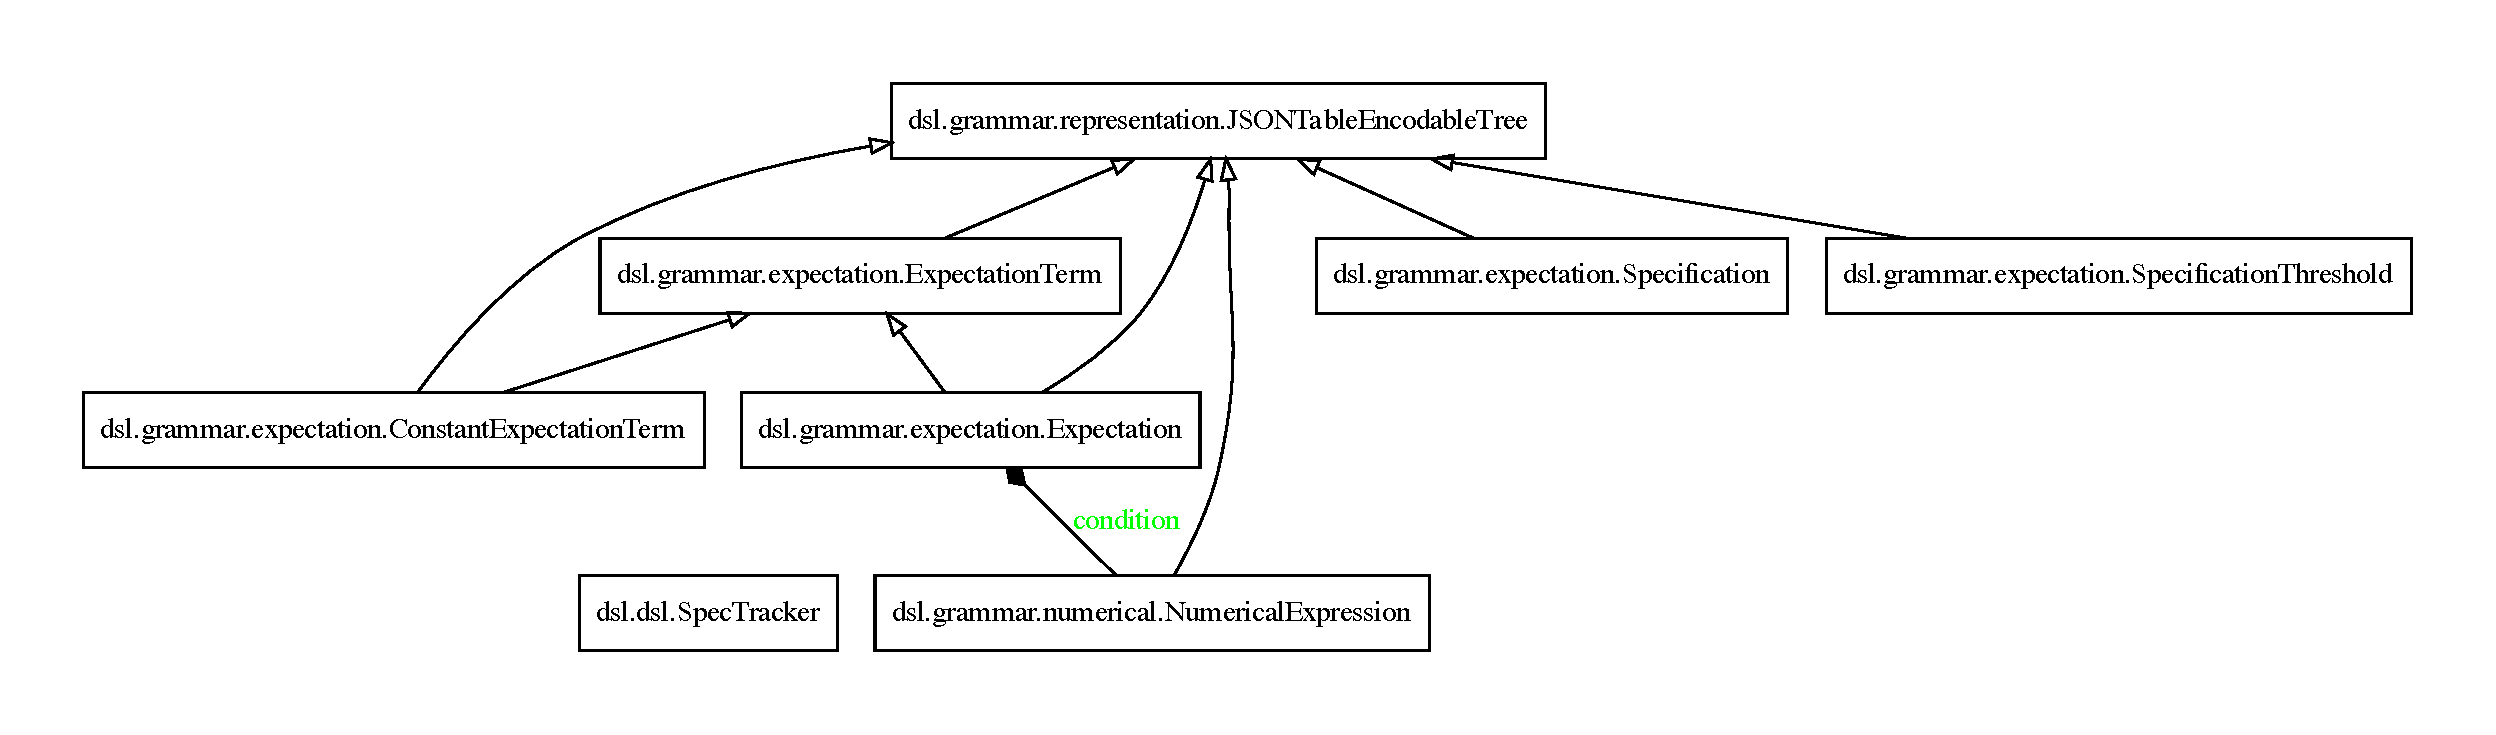
\includegraphics[width=\linewidth]{class-diagram.pdf}
    \caption{Diagram for the internal class structure of implementation}
    \label{fig:class-diagram}
\end{figure*}

Our long-term goal is to support automated transformations to specifications.
Given a specification and dataset statistics from the running it on data, we should be able to generate suggestions for better, related specifications to guide a user towards a situation appropriate fairness metric. 
One mechanism to support such transformations would be to construct a custom domain specific language (DSL) parser and perform edit operations on the extracted syntax tree from a parsed specification.
Our implementation takes a different route - we implemented the entire DSL using python. 
That is, each non-terminal expressible in the modified grammar corresponds to a unique python object. 
We construct classes to represent each of these objects and overload the appropriate operators such that any statement in the python version of the DSL corresponds to a unique statement in the modified grammar. 
Figure~\ref{fig:class-diagram} shows an overview of the python implementation. 

\newcommand{\NE}{\texttt{NE}}
\subsubsection{\texttt{NumericalExpression} (\NE)}
The \NE class is used to construct pure expressions $\langle E \rangle$ in the grammar.
An \NE{} is an (at most binary) expression consisting of python variables and constants with arithmetic/relational operators applied to them.
At run time, the parameters from the decision function are bound to the corresponding variable in each \NE{} and then then its value is computed using python's own internal operators. 
A reserved string represents the \NE{} corresponding to the return value of the decision function.
The utility function \texttt{create\_variable} is provided to create bindings from formal parameters of functions to a variable \NE. 
Thus, declaring a variable corresponding to a formal parameter of a decision function is as simple as 
\begin{lstlisting}[language=python]
from dsl.grammar.NumericalExpression \
    import create_variable as V
V("sex")
\end{lstlisting}

\noindent this creates an \NE{} for the `sex' variable given as part of the input to a decision function. 
Additionally, we coerce the type of integer and float constants to \NE{} for ease of use, e.g., making expressions such as \texttt{V('height')/2} usable within a spec without explicitly defining \texttt{2} as a constant \NE{}. 

\newcommand{\ET}{\texttt{ET}}
\subsubsection{ExpectationTerm (\ET)}
represented by $\langle ETerm \rangle$ in the grammar, denote the expected value of a numerical expression, a conditional expectation, a constant, or binary composition of two \ET{}.
We use sub-classes \texttt{ConstantExpectationTerm} and \texttt{Expectation} to capture these different kinds of expectation terms. 

\subsubsection{SpecificationThreshold} denotes a wrapped base level specification.
In the grammar, this corresponds to $\langle ETerm\ \rangle\ \langle\ comp-op\ \rangle\ c$. 
All \texttt{SpecificationThreshold} terms are wrapped by a\\ \texttt{Specification}, but we maintain these as separate classes for semantic reasons. 
To further improve the ease of use, we overload the comparison operators for \ET{} to type coerce any binary boolean expression of an $\langle ETerm \rangle$ to a \texttt{SpecificationThreshold}.  

\subsubsection{Specification} is the top level specification class. 

\subsubsection{JSONTableEncodableTree} is a special class that provides methods that all subclasses must override. 
The overridden methods control the JSON representation of the class, which is used for generating nodes in the Vega visualization tree. See Section~\ref{sec:implementation:vis} for details of the visualization. 

\subsubsection{SpecTracker} Specification tracking is implemented by a decorator \texttt{@spec}, which wraps a decision function in code that passes the arguments and return value to the specification corresponding to each decision function.
The \texttt{SpecTracker} class maintains a dictionary which links each function to its corresponding specification and also a global invocation timestamp. 
The actual values of each individual term in the specification are maintained by the objects that constitute the specification.
The global timestamp values help generate line plots of each term over time and compare the values of different terms at the same point of time. 

% definitions to make the math easier to type
\newcommand{\Eb}{\bar{E}}
\newcommand{\eps}{\epsilon}

\subsection{Probabilistic Guarantees}
\label{sec:implementation:prob}
Section~\ref{sec:implementation:framework} describes the implementation details that improve the expressiveness and usability of the grammar. 
However, the current implementation only supports the generation of point estimates for each (sub)term within a specification. 
\citet{albarghouthi2019fairness} augment the point estimate by a probabilistic estimate by reporting a violation iff the probability of failure $> \kappa$, where $\kappa$ is a user specified threshold. 
The use case for our tool is as an aid to the design of the specification itself. 
Thus, we aimed to provide a probabilistic guarantee.
We refined the estimates from previous work to improve the probabilistic bounds and augment the point estimate of the specification (and sub-terms) with minimum guaranteed probabilities.
Concretely, given a specification $\E[X] > c$, we report whether $\bar{E} > c$, and $\p(\E[X] > c)$ or $\p(\E[X] \leq c)$. 
Here, $\bar{E}$ is the empirical point estimator for $\E[X]$, and $X$ is a pure expression.
We then describe how this bound can be extended to compound specifications that contain some binary expression of specification. 
We conclude with an illustration of how the same bounds can be derived for any compound $\langle ETerm \rangle$ that involves numerical operations across multiple elementary $\E$.

\subsubsection{Elementary Assertions}
\label{sec:implementation:prob:elem}
For the remainder of this section, we will assume that $\bar{E} > c$.
Similar bounds can be derived for the alternative case. 
We have
\begin{align*}
\p(\E[X] > c) &\geq \p(2\bar{E} - c > \E[X]  > c ) \\
                    & = \p (\bar{E} -c > \E[X] - \bar{E} > c - \bar{E}) \\
                    & = \p(|\bar{E}-\E[X]| < \bar{E} - c)  \\
                    &= 1 - \p(|\bar{E} - \E[x]| \geq \bar{E} - c)
\end{align*}
Using concentration inequalities of the form
\begin{equation}
    \p(|\bar{E} - \E[X]| \geq \epsilon) \leq \delta
    \label{eq:conc-ineq}
\end{equation}
and substituting $\epsilon = \bar{E} - c$ in equation~(\ref{eq:conc-ineq}), we can derive 
\begin{align*}
    \p(\E[X] > c) &\geq 1 - \p(|\bar{E} - \E[x]| \geq \bar{E} - c) \\
        & \geq 1 - \delta
\end{align*}
which gives us a upper bound probability for the failure of an elementary assertion.

\subsubsection{Compound Assertions}
\label{sec:implementation:prob:comp}
In this section, we demonstrate an algorithm that can be used for the binary addition of two $\langle ETerm \rangle$. 
However, the same arguments can be extended to the other operators, with appropriate modifications to the cumulative $\epsilon$ and $\delta$ terms.
Suppose we want to compute a bound on the failure probability of the assertion
\begin{align*}
    \E[E_1] + \E[E_2] > c
\end{align*}
Let $\delta_1$ and $\delta_2$ denote the estimated failure probability for $\E[E_1]$ and $\E[E_2]$, and $\epsilon_1$, $\epsilon_2$ denote the deviation from their point estimates $\bar{E}_1$ and $\bar{E}_2$ (i.e, $P(|E[X_i] - \bar{E}_i| \geq \epsilon_i) \leq \delta_i$). 
Suppose $\delta_{12}$ denotes the failure probability of $\p(\E[E_1] + \E[E_2] > c)$, and $\epsilon_{12}$ be the combined deviation from the mean.
From \cite{albarghouthi2019fairness}, we have 
\begin{align*}
    \delta_{12} &= \delta_1 + \delta_2 \\
    \epsilon_{12} &= \epsilon_1 + \epsilon_2
\end{align*}
We want to minimize the failure bound $\delta_{12}$ in our estimates.
Using the constraint on $\epsilon$ derived in section~\ref{sec:implementation:prob:elem}, we can express this as the optimization 
\begin{align*}
    &\min{\delta_1 + \delta_2} \\
    \text{s.t.  } &\epsilon_1 + \epsilon_2 < \bar{E}_1 + \bar{E}_2 - c\\
    & 0\leq \delta_i \leq 1
\end{align*}
Let $\delta_i = f_i(\epsilon_i, n_i, E_i, \bar{E}_i, \dots) = f_i(\epsilon_i)$ be the function that relates $\epsilon_i$ with $\delta_i$, given the expression, observations associated with it so far, and relevant concentration inequality. Assuming that $f_i$ is invertible, and substituting $\eps_{12} =  \bar{E}_1 + \bar{E}_2 - c$ we have
\begin{align*}
     &\min{\delta_1 + \delta_2} \\
    \text{s.t.  } & f_1^{-1}(\delta_1) + f_2^{-1}(\delta_2) < \eps_{12}\\
    & 0\leq \delta_i \leq 1
\end{align*}

Further, assuming that $f_i^{-1}$ are convex and differentiable, \textcolor{red}{it can be shown that} the feasible region $f_1^{-1}(\delta_1) + f_2^{-1}(\delta_2) < \eps_{12}$ is convex, the boundary is a monotonically non-decreasing function and thus, the derivative of the boundary is a one-one function~\cite{bertsekas1997nonlinear}. 
Let the feasible set  $C = \{(\delta_1, \delta_2)| f_1^{-1}(\delta_1) + f_2^{-1}(\delta_2) < \eps_{12}  \}$
A solution $(\delta_1^*, \delta_2^*)$ is optimal iff $(\delta_1^*, \delta_2^*) \in C$ and 
\begin{align*}
    \nabla(\delta_1 + \delta_2)_{(\delta_1^*, \delta_2^*)}^T(\delta_1 - \delta_1^*, \delta_2 - \delta_2^*) \geq 0
\end{align*}
$\forall \delta_1, \delta_2 \in C$~\cite{bertsekas1997nonlinear}. Simplifying,

\begin{equation}
\delta_1 + \delta_2 \geq \delta_1^* + \delta_2^*    
\label{eq:optimality-cond}
\end{equation}

Consider the family of curves $L = \{\delta_1 + \delta_2 = c\}$, $c\in \mathbb{R}$. 
Let the boundary of $C$ be $C_b$.
The derivative of $C_b$ is a one-one function, therefore it must have a unique tangent $\in L$, and the point of intersection of this tangent with $C$ will satisfy the optimality condition from equation~\ref{eq:optimality-cond}. 
Thus, we must construct an algorithm to find this intersection. Figure~\ref{fig:optimization-demo} shows a pictorial representation of the aforementioned condition. 

\subsubsection{Other compound assertions}

\begin{itemize}
    \item For the assertion $\E[E_1] - \E[E_2] > c$ the proof follows the same arguments as the case fo the $+$ operator, and is provided here for completeness,
    \begin{align*}
        &\min{\delta_1 + \delta_2}\\
        \text{s.t, }  &\Eb_1 \pm \eps_1 - (\Eb_2 \pm \eps_2) > c\\
        & 0 \leq \delta_i \leq 1
    \end{align*}
    and since $\eps_1, \eps_2 \geq 0$, setting $(\Eb_1 - \Eb_2) - c = \eps_{12}$, we get the inequality $\eps_1 + \eps_2 < \eps_{12}$
    \item For the assertion $\E[E_1] * \E[E_2] > c$. In the failure cases, we have $E_i > \Eb_i + \eps$ or $E_i < \Eb_i - \eps$. Thus, the overall optimizaiton problem is
    \begin{align*}
        &\min{\delta_1 + \delta_2} \\
        \text{s.t, } &\Eb_1 \Eb_2 + \eps_1 \eps_2 -\eps_1\Eb_2 - \eps_2\Eb1 > c\\
        &\Eb_1 \Eb_2 - \eps_1 \eps_2 + \eps_1\Eb_2 - \eps_2\Eb1 > c \\
        &\Eb_1 \Eb_2 - \eps_1 \eps_2 - \eps_1\Eb_2 + \eps_2\Eb1 > c\\
        &\Eb_1 \Eb_2 + \eps_1 \eps_2 + \eps_1\Eb_2 + \eps_2\Eb1 > c\\
        &0 \leq \delta_i \leq 1
    \end{align*}
    with $\Eb_1\Eb2 - c = \eps_{12}$, we have
    \begin{align*}
        &\min{\delta_1 + \delta_2} \\
        \text{s.t, } & - \eps_1 \eps_2 +\eps_1\Eb_2 + \eps_2\Eb1 < \eps_{12}\\
        &  \eps_1 \eps_2 - \eps_1\Eb_2 + \eps_2\Eb1 < \eps_{12} \\
        &  \eps_1 \eps_2 + \eps_1\Eb_2 - \eps_2\Eb1 < \eps_{12}\\
        & -\eps_1 \eps_2 - \eps_1\Eb_2 - \eps_2\Eb1 < \eps_{12}\\
        &0 \leq \delta_i \leq 1
    \end{align*}
    \item For the assertion $\E[E_1]/\E[E_2] > c$, we need $\frac{\Eb_1 \pm \eps_1}{\Eb_2 \pm \eps_2}$. Setting $c - \frac{\E[E_1]}{\E[E_2]} = \eps_{12}$,
\end{itemize}

\begin{figure}
    \begin{tikzpicture}
        \begin{axis}[
                %xtick = \empty,    ytick = \empty,
                grid=both,
                xlabel = {$\delta_1$},
                x label style = {at={(1,0)},anchor=west},
                ylabel = {$\delta_2$},
                y label style = {at={(0,1)},rotate=-90,anchor=south},
                axis lines=left
            ]
            \addplot[name path=f,color=red,smooth,thick,-,domain=0:1] {x/(10(x)^0.5-1)^2};
            \addlegendentry{$C_{b}$}
            
            \addplot[mark=none, blue, domain=0:0.5] {0.5-x};
            \addlegendentry{$\delta_1 + \delta_2 = \delta_{12}^*$}
            
            \path[name path=axis] (axis cs:0,1) -- (axis cs:1,1);
            
            \addplot[
                thick,
                color=red,
                fill=red,
                fill opacity=0.05
            ]
            fill between[
                of=f and axis,
                soft clip={domain=0:1}
            ];
            \addlegendentry{$C$}
            \addplot[dotted,color=blue,thick,smooth,domain=0:0.8]{0.8-x};
            \addplot[dotted,color=blue,thick,smooth,domain=0:0.2]{0.2-x};
            %\draw[fill=red!50]
        \end{axis}
    \end{tikzpicture}
    \caption{Plot showing the feasible region $C$, its boundary $C_b$, the unique tangent $\delta_1 + \delta_2 = \delta_{12}^*$. The blue dotted lines show non-optimal lines inside and outside the feasible region.}
    \label{fig:optimization-demo}
\end{figure}

\subsubsection{Algorithm for Optimal Solution}
We propose a binary search based algorithm to find the optimal intersection. 
The idea is to search over candidate $l_t \equiv \delta_1 + \delta_2 = t \in L$, and solve the simultaneous pair of equations for $l_t$ and $C_b$. 
If we find any feasible solution, then the tangent must be a curve $l_{t'}$  with $t' \in (0, t]$.
If there is no solution, then the tangent must be a curve $l_{t'}$ with $t' \in (t, 1]$.
This idea can easily be instantiated into a binary search based procedure to find the optimal $t$, with an initial range of $t\in (0, 1]$. 

\subsubsection{Concentration Inequalities}
For deriving the above algorithm, we have assumed that $f_i$ will be an invertible function with a convex, differentiable inverse. 
Here, we verify this for the Chebyshev inequality. 

\begin{align*}
    \p(|X-\E[X]| \geq \epsilon) \leq \frac{Var(X)}{\epsilon^2}
\end{align*}
Substituting the empirical mean as $X$, and simplifying, we get 
\begin{align*}
    f(\epsilon) &= \frac{Var(X)}{n\epsilon^2}\\
\implies f^{-1}(\delta) &= \sqrt{\frac{Var(X)}{n\delta}} = k_c\sqrt{\frac{1}{\delta}}
\end{align*}
for an appropriate constant $k_c$. In the domain $0\leq\delta\leq 1$, this function is convex.
We note that similar results can also be derived for other inequalities such as the Hoeffding inequality, but omit the detailed derivation here. 





 \begin{comment}
 \subsection{Implementation}
 \label{sec:specification:implementation}
 Short section on how the grammar is implemented based on the text in comments.tex with additional details about DB/Pandas
 \end{comment}